\documentclass[Bachelorarbeit.tex]{subfiles}
\begin{document}
\chapter{Results}

In this Chapter the results of the experiments are given. Each topology-type is handled in a separate section where the hypothesis was put to test in the section regarding the Ascending-Connected Topologies.

In all experiments 100 Agents were used, all markets were enabled, the bond-type 0.5 was selected and if replications were used the number of runs over which was averaged was always 50.
As Termination-Mode "Failed successive Transactions" is selected with the number of failed transactions in a row is 1000. Note that if trading is not possible anymore bevore these 1000 failed transactions have been reached, the simulation is halted and thus it is possible that it terminates earlier.

100 agents were chosen because \cite{Breuer2015} showed that equilibrium can be reached already with 30 agents so this was the minimum number of agents to start with. For a finer "resolution" of the visual results 100 were chosen also because its a good match between too much processing power required and nice visual results.
The 0.5 Bond was selected because its a risky one and only when a risky bond is traded then will this equilibirum show up as for unrisky bonds with Facevalue <= 0.2 the results are indifferent.
Obviously the whole simulation-process is a random-process with an equilibrium (different for each topology) as the fixed-point solution thus one needs replications to reduce noise. The number of 50 Replications was chosen because its a good match between run-time duration and overall reduction of noise - increasing the number e.g. to 100 or 200 would not result in much better results but would need much longer to run. All facts can be seen and derived when using 50 replications.

Theoretical equilibrium for i0, i1, asset price and loan price can be calculated and are as follows:

\begin{tabular} { l c r }
	Asset-Price (p) & 0.716 \\
	Loan-Price (q) & 0.384 \\
	Asset/Loan Price (pq) & ? \\
	Marginal Buyer i0 & 0.584 \\
	Marginal Seller i1 & 0.801 \\
\end{tabular}



\section{Fully-Connected Topology}
To demonstrate the ability of the software to produce the results given in the paper of \cite{Breuer2015} the results of a single run and in addition with a replication run of a Fully-Connected Topology is given.

It is also a point-of-reference for the other experiments as this fully-connected topology gives a good point of visual information which can be applied to the other topologies to give a visual clue whether they could have actually reached the equilibrium.

\begin{figure}[ht]
	\centering
  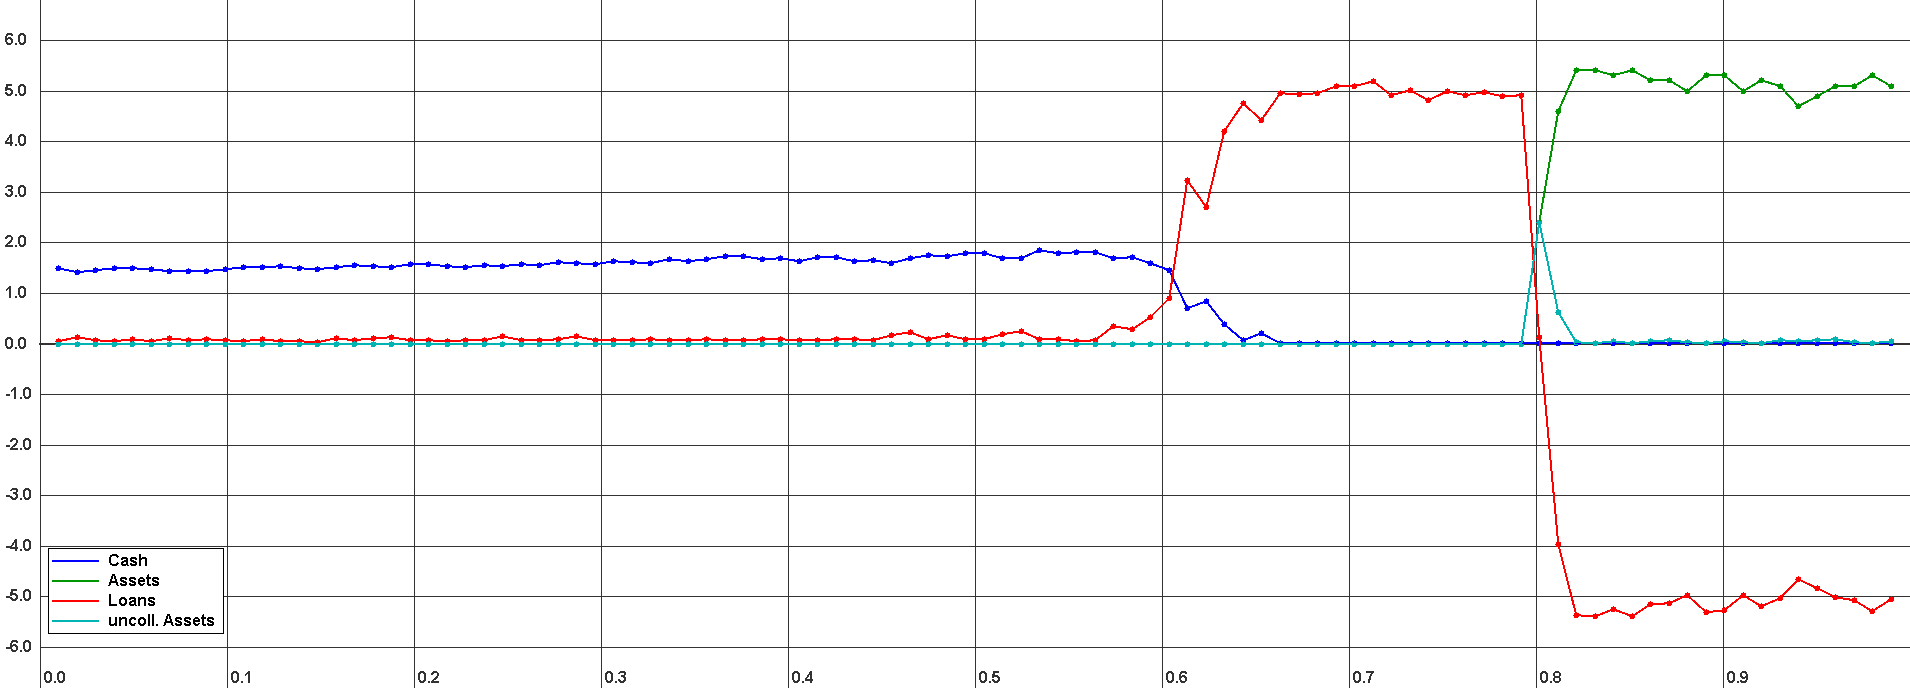
\includegraphics[width=1.0\textwidth, angle=0]{FULLYCONNECTED_100_NOCOLLATERALMARKET_SINGLE.png}
	\caption{Fully-Connected topology wealth-distribution after single run}
	\label{fig1}
\end{figure}

\begin{figure}[ht]
	\centering
  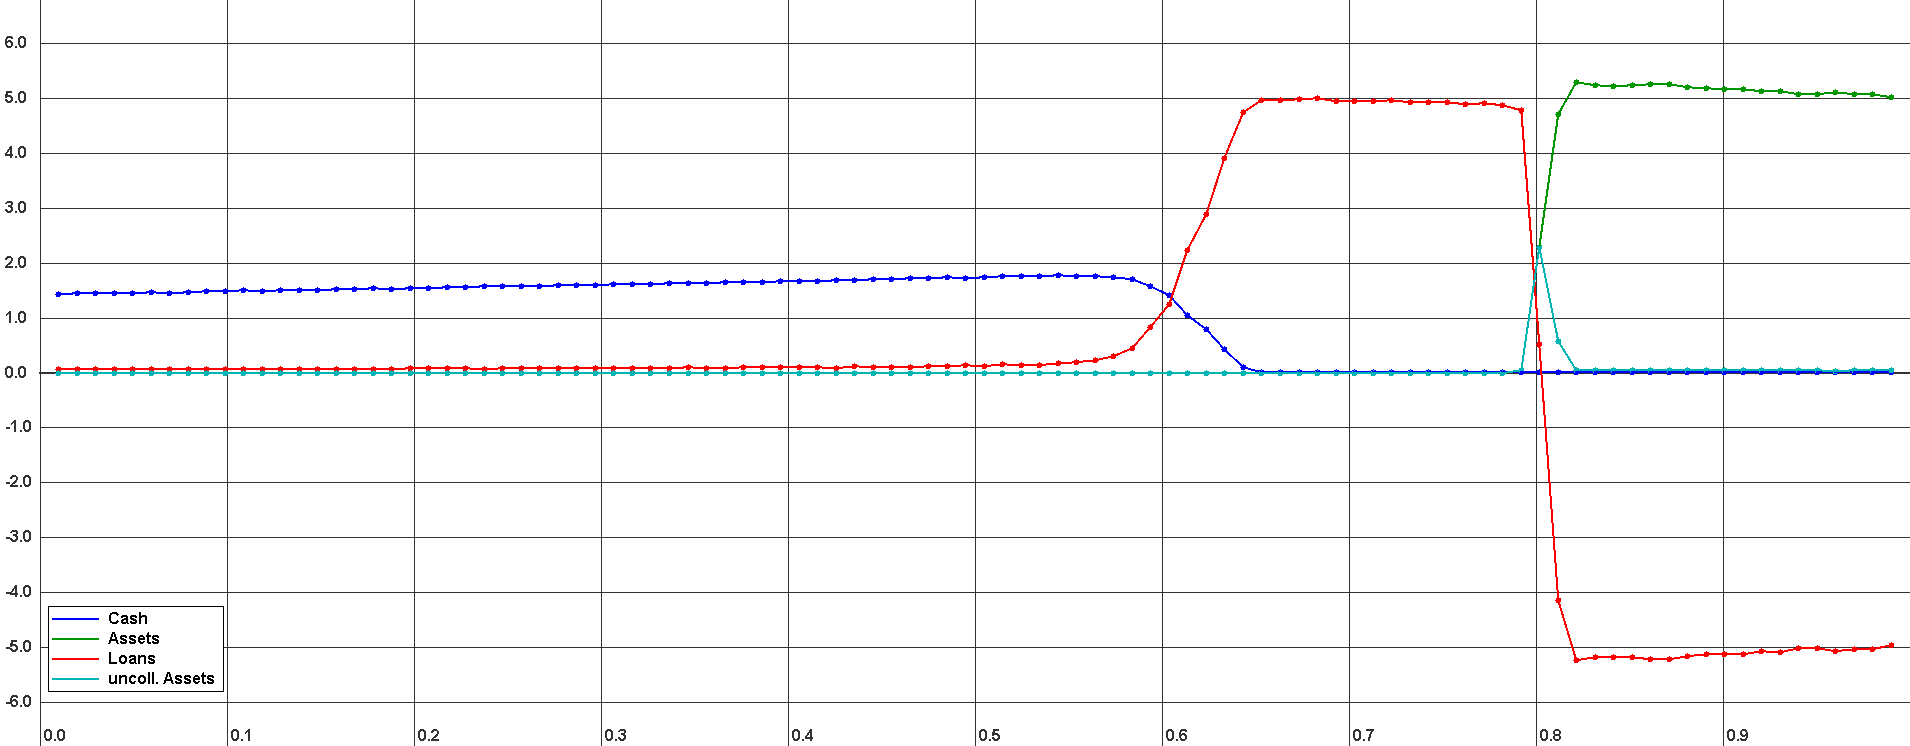
\includegraphics[width=1.0\textwidth, angle=0]{FULLYCONNECTED_100_NOCOLLATERALMARKET_REPL.png}
	\caption{Fully-Connected topology wealth-distribution after 50 replications}
	\label{fig1}
\end{figure}

Equilibrium (Standard-deviations are given in parantheses)

\begin{tabular} { l c r }
	Asset-Price & 0.689 (0.010) \\
	Loan-Price & 0.384 (0.004) \\
	Asset/Loan Price & 1.911 (0.001) \\
	i0 (Marginal Buyer) & 0.603 (0.007) \\
	i1 (Marginal Seller) & 0.803 (0.003) \\
	Pessimist Wealth & 1.597 (0.015) \\
	Medianist Wealth & 4.565 (0.113) \\
	Optimist Wealth & 5.021 (0.064) \\
\end{tabular}

Performance (Standard-deviations are given in parantheses)

\begin{tabular} { l c r }
	Successful TX & 1916.14 (31.42) \\
	Total TX & 6364.8 (1679.21) \\
	Failed TX & 4448.66 (1668.93) \\
\end{tabular}



\section{Ascending-Connected Topologies} 

\subsection{Ascending-Connected}

\subsection{Ascending-Connected Importance Sampling}

\subsection{Ascending-Connected 5 full Short-cuts }
\subsection{Ascending-Connected 15 full Short-cuts }
\subsection{Ascending-Connected 30 full Short-cuts }

\subsection{Ascending-Connected 5 regular Short-cuts }
\subsection{Ascending-Connected 15 regular Short-cuts }
\subsection{Ascending-Connected 30 regular Short-cuts }



\section{Deterministic Hub-Based Topologies} 

\subsection{Half-Fully Connected}
\subsection{3-Hubs}
\subsection{1-Median Hub}
\subsection{3-Median Hub}
\subsection{Maximum Hub}



\section{Random-, Scale-Free and Small-World Topologies}
\subsection{Ascending-Connected random Short-cuts}
\subsection{Erdos-Renyi}
\subsection{Barbasi-Albert}
\subsection{Watts-Strogatz}

\end{document}
